\documentclass[a4paper]{article}
\usepackage{datetime}
\newdate{date}{13}{09}{2022}
\date{\displaydate{date}}

%% Language and font encodings
\usepackage[english]{babel}
\usepackage[T1]{fontenc}
\usepackage{float}

%% Sets page size and margins
\usepackage[a4paper,top=3cm,bottom=2cm,left=3cm,right=3cm,marginparwidth=1.75cm]{geometry}

%% Useful packages
\usepackage{notes2bib}
\usepackage{textcomp}
\usepackage{amssymb}
\usepackage{amsmath}
\usepackage{graphicx}
\usepackage[colorinlistoftodos]{todonotes}
\usepackage[colorlinks=true, allcolors=blue]{hyperref}

\title{Week 3 Assignment-Journal}
\author{Dustin J. Trujillo}

\begin{document}
\maketitle

%%\begin{abstract}
%%To be added later.
%%\end{abstract}

\section{Part 1: 'Denial of Service' Research Direction}
My initial research direction/query is "denial of service" AND survey. I searched Google Scholar for the past six years (2017-2022). I broke up my search into year by year for each of these years and quickly browsed/scanned for any result that appeared to be a survey paper and was relevant to my research direction. As you can see from the bibliography (it includes papers that I cited here as well as the papers I did not cite), I found quite a few (48 in total) surveys related to Denial of Service that were published during this six year period.

\section{Part 2: Search and Survey Results}
Of the 48 survey papers, I critically/creatively read four of them \cite{mahjabin2017survey, saif2018review, salim2020distributed, rios2022detection}, and put short notes for each of them. Below are the notes  from my critical and creative reads and to the highest and lowest cited reasons: \\

This paper \cite{mahjabin2017survey} is from 2017 is the highest cited paper (with 229 citations) of all the surveys (2017-2022). I believe it is the highest cited paper in part, because it also one of the oldest papers in the search period, but also because the paper is more than just a summary: it compares and contrasts others, has a theme and a goal, helps organize ideas, and the authors also add additional and new insights. \\

Here are my raw notes from \cite{mahjabin2017survey}:\\
A SURVEY OF DDoS ATTACK, PREVENTION, AND MITIGATION TECHNIQUES

1. Seven Ws about the survey example (Who, What, When, Where, Why, for Whom, hoW): Good authors and publication.


2. Essence (it can extremely difficult to give entire essence in only one sentence): The authors present a comprehensive survey of DDoS attack, prevention, and mitigation techniques.

3. Structure: Introduction, Attack Targets and Motivations, Attack Strategies, Attack Phases (scanning, propagation, attack attempt), attack mechanisms, attack types, and attack on nontraditional systems (clouds, smart grids, smart homes, CPSs, and IoT systems). Recommended other areas of research.

4. Some relevant details: A response to the 2016 uptick in DDoS attacks.

5. Example (here one can call a figure that explains an example using a pseudo-code;  ideally, the same application case should be used for all surveyed examples): Figure 1 shows volume sizes in DDoS attacks from 2007-2016.

6. Pros and cons: 
PRO They cover nearly (if not all) DDoS attack types known at the time of the writing (2017). 
PRO Really good future suggestions for research:
1.  All recent major DDoS attacks are based on IoT botnets- Prevent creation of the IoT botnets, detection, and rejection of the flows from unsophisticated IoT devices (such as security camera, smart refrigerator, home routers).
2. Ensure the lowest possible consumption of the victim’s resources by the defense mechanisms while fighting against DDoS.
3. Scalabiilty: It is very important to test the real-life performance of those researches.
4. Ensure defense against Zero days.

7. My opinion of this example and its potentials: Very good paper, no wonder why it is top cited. Directions for other research are very good. 
\\

This paper \cite{saif2018review} is from 2018 and is the lowest cited paper (with one citation) of all the surveys (2017-2022). I believe it is the lowest cited paper because it just summarizes some of the literature and does not compare of contrast. The topic (transport layer) may also be too narrow and not very interesting to the larger community. Additionally, this paper may have been shortened as it appears to have been from a conference and is only five pages long. \\

Here are my raw notes from \cite{saif2018review}:\\
RECENTLY EMERGING DENIAL OF SERVICE THREATS AND DEFENCES IN THE TRANSPORT LAYER

1. Seven Ws about the survey example (Who, What, When, Where, Why, for Whom, hoW): was from 2018 IEEE Canadian conference.

2. Essence (it can extremely difficult to give entire essence in only one sentence):Cover the latest strides in attack methodologies and related defence mechanisms specific to the Transport layer.

3. Structure: Intro, Related Work, Attack and Defence Taxonomy, Emerging Attack Types.

4. Some relevant details: Author doesn't create a new taxonomy, only simply uses it to highlight new trends.

5. Example (here one can call a figure that explains an example using a pseudo-code;  ideally, the same application case should be used for all surveyed examples): Didn't really have any good figures.

6. Pros and cons: Has good tables to define attack and defense metrics. Very short paper, likely due to it being from a conference.

7. My opinion of this example and its potentials:
Was not able to find the actual longer/non conference version of the paper. It was useful in the sense that it referred to an existing taxonomy, but this paper did not really evaluate in depth the previous work and take it to the next level. Also, the topic may have been very narrow, hence the lack of citations.\\

Here are my raw notes from \cite{salim2020distributed}:\\
DISTRIBUTED DDOS AND DEFENSES IN IOT (CLOUD)

1. Seven Ws about the survey example (Who, What, When, Where, Why, for Whom, hoW): Reputable journal, university and authors.

2. Essence (it can extremely difficult to give entire essence in only one sentence): Focuses on  motivations and reasons for attackers to select non-legacy IoT devices to launch DDoS attacks.

3. Structure: Introduction, Motivations for attackers to use non-legacy IoT devices, single vs multi vector attack patterns, taxonomy, defense mechanisms, suggestions.

4. Some relevant details: Focuses on  motivations and reasons for attackers to select non-legacy IoT devices to launch DDoS attacks.

5. Example (here one can call a figure that explains an example using a pseudo-code;  ideally, the same application case should be used for all surveyed examples): Fig. 2 current form of multi-vector DDoS attacks.

6. Pros and cons:
PRO A complete survey of DDoS attacks for both IoT and the cloud environment which was not present in the current literature.
PRO Ties research to Mirai/Reaper Botnet which used 148,000 infected IoT devices.
PRO DDoS Cloud Classifications


7. My opinion of this example and its potentials: Does a good job bringing together two areas with lots of research that hadn't been presented together before (IoT and cloud). Very comprehensive. Provides suggestions on how to defend.
CON: didn't really list areas for future research.\\

Here are my raw notes from \cite{rios2022detection}:\\
DETECTION AND MITIGATION OF LOW RATE DENIAL OF SERVICE ATTACKS: A SURVEY

1. Seven Ws about the survey example (Who, What, When, Where, Why, for Whom, hoW): Well established authors, mostly Member or Senior IEEE members.

2. Essence (it can extremely difficult to give entire essence in only one sentence): Summarizes and complements previous studies and surveys related to this specific type of attack.

3. Structure:
A. Propose a taxonomy of the LDoS attacks, (divided into three
broad categories based on their modus operandi: QoS attacks, Slow rate attacks, and Service queue attacks)
B. Detail numerous detection mechanisms and counter-measures available against eight types of LDoS
attacks (i.e. Throttle)
C.Provide a feature comparison table for some existing attack tools. 

4. Some relevant details: Focuses on Low Rate DoS attacks.

5. Example (here one can call a figure that explains an example using a pseudo-code;  ideally, the same application case should be used for all surveyed examples): Lots of Figures and Tables useful for attack patterns and taxonomy

6. Pros and cons:
PRO Aims at providing an extensive review of the literature for helping researchers and network administrators find up-to-date knowledge on LDoS attack.
PROS: Table and taxonomy very useful
PROS: Seems to have brought together all of the existing research and develop all the tables and figures for quick reference.
CONS: doesn't provide suggestion on future areas of work.

7. My opinion of this example and its potentials: Useful for helping researchers and network administrators find up-to-date knowledge on LDoS attacks. 
CON: doesn't provide suggestion on future areas of work.

\section{Part 3: Topic Map}
As mentioned previously, in the bibliography I listed all the relevant Denial of Service surveys that were published during 2017-2022. I began my Topic Map by scanning all of the 48 surveys to get a "lay of the land" for all the different sub areas of Denial of Service. See Figure 1 for the Denial of Service Topic Map.

\begin{figure}[H]
\centering
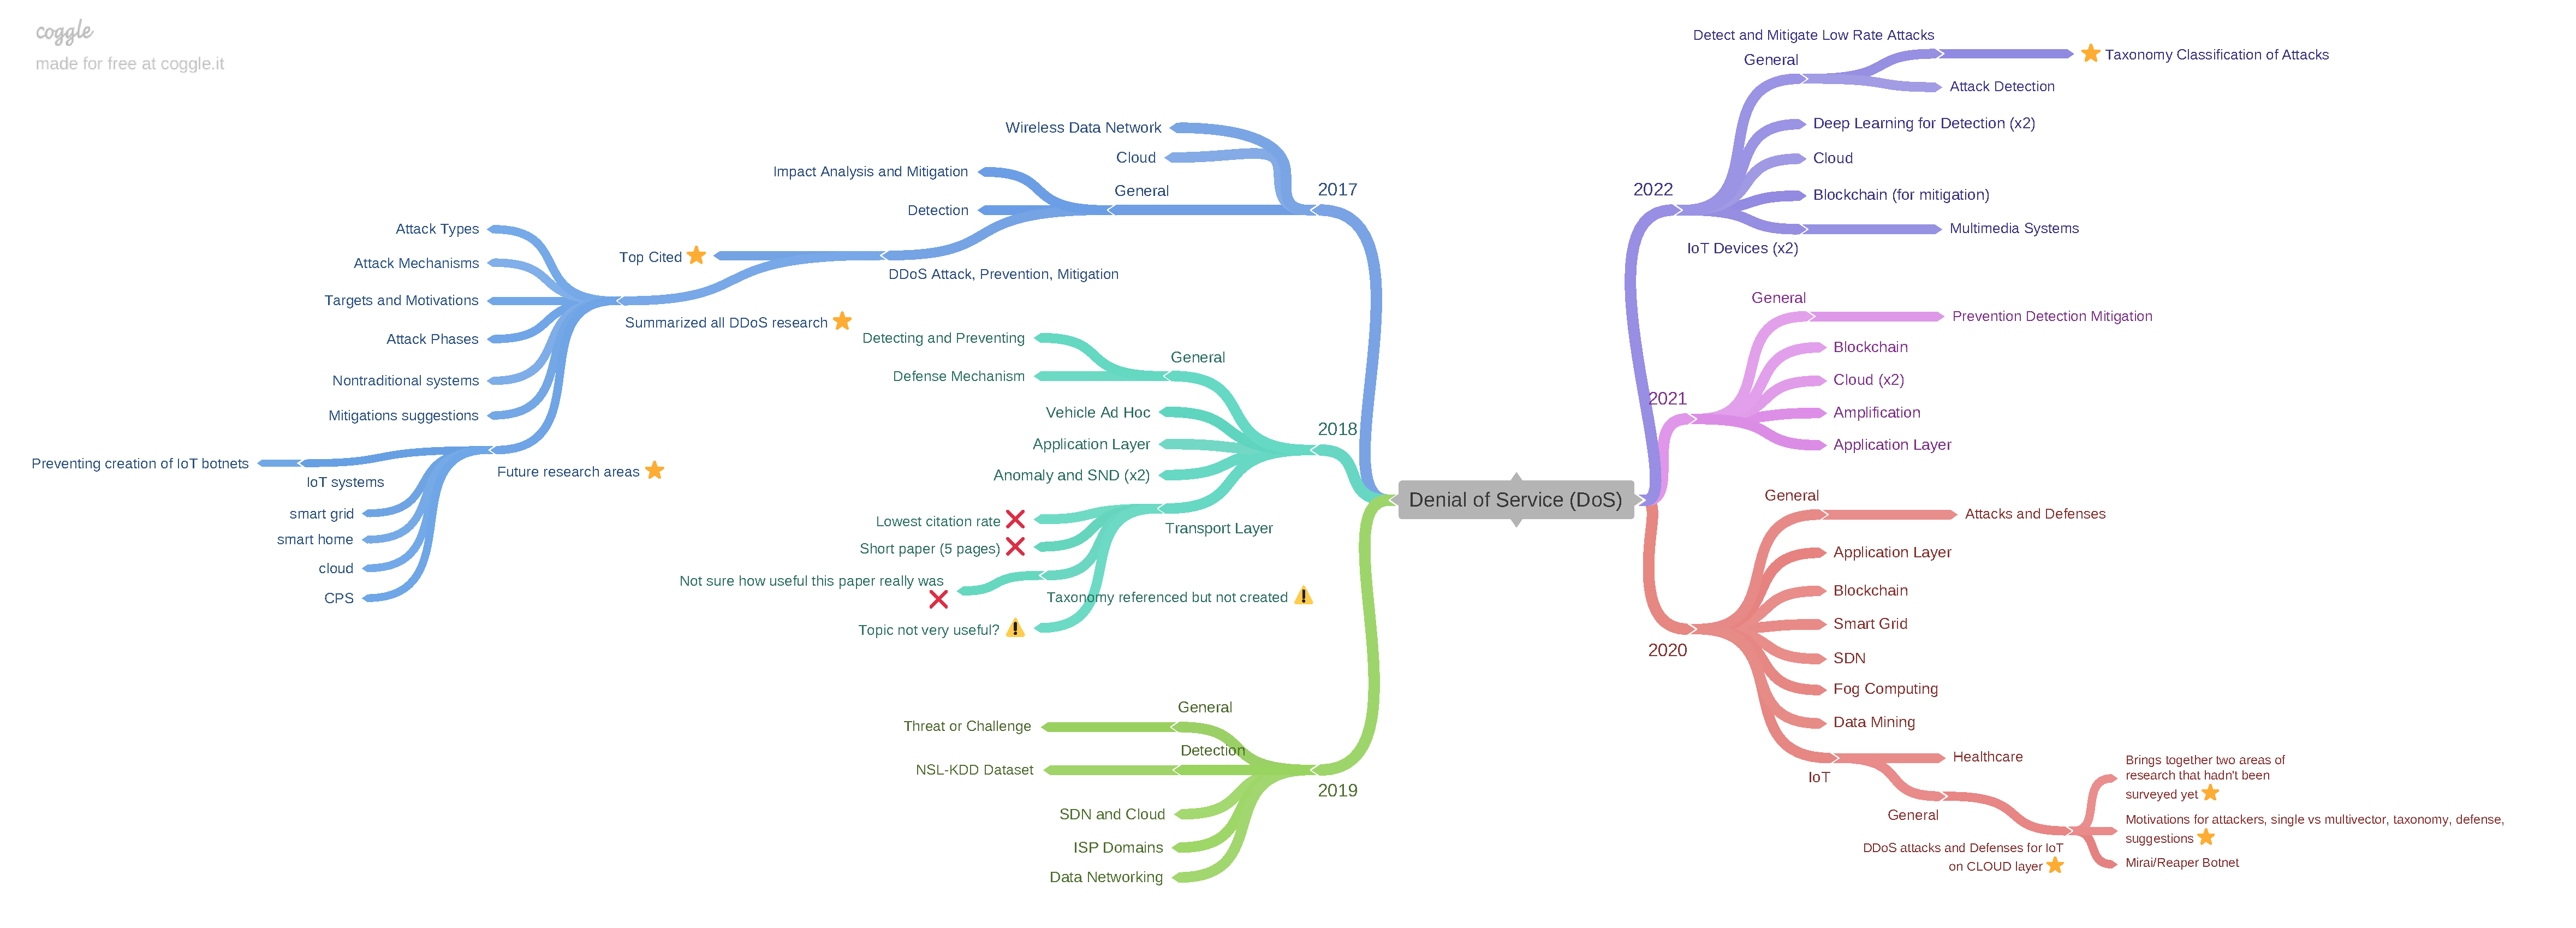
\includegraphics[width=1\textwidth]{Denial_of_Service_DoS.pdf}
\caption{\label{fig:DOS}Denial of Service Topic Map}
\end{figure}

 As you can see from Figure 1, all major sub areas of the 48 survey papers are noted/listed by year. However, you will see one area in 2017 (DDoS Attack, Prevention, Mitigation), one in 2018 (transport Layer), one in 2020 (DDoS attacks and Defenses for IoT on CLOUD layer), and one in 2022 (Detect and Mitigate Low Rate Attacks), where I continued breaking out the topic areas. These four areas are also areas from the four surveys that I did the critical/creative read on. What's more, drom these four surveys, I notated the red Xs on the topic map to indicate items to avoid when developing my own survey paper, and the yellow stars to indicate gaps in existing surveys and possible areas for future research/surveys.

\section{Part 4: Public git-repo}

I have also made my Overleaf LaTeX/Project file into a public github repo and It can be found here: \href{https://github.com/dustbonetru/Week-3-Assignment-Journal}{Dustin's Week 3 Assignment-Journal}. In the github repo, you can open the main.tex to see the main journal entry. All other files are supporting files.

\nocite{*}
\bibliographystyle{IEEEtran}
\bibliography{w3bibliography.bib}

\end{document}